% Appendix A

\chapter{Additional Plots}\label{AppendixA}

\begin{figure}[h]
  \centering
  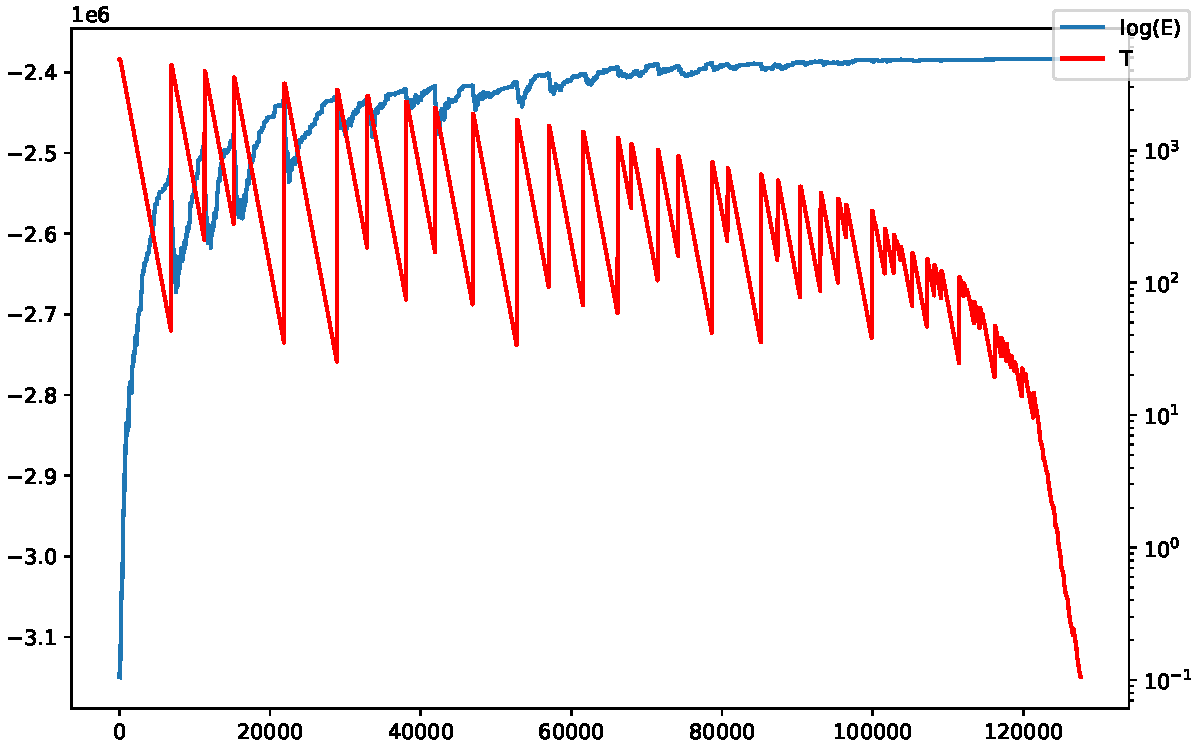
\includegraphics[width=\textwidth]{./Figures/Adaptive_trace.pdf}
  \caption{The history of the \loge{} during the best run of the adaptive annealing algorithm. This algorithm had a decay rate of 0.001 and a reset factor of 0.95. The blue line shows the \loge{}, and the red line the logarithm of the temperature.}\label{adaptTrace}
\end{figure}